\documentclass{article}
\usepackage{graphicx}
\usepackage{fancyhdr}
\usepackage{lipsum}
\usepackage[margin=1in]{geometry} % Set margins to 1 inch


% Header configuration
\pagestyle{fancy}
\fancyhf{}
\fancyhead[L]{
\includegraphics[height=20pt]{image/usl_logo.png}}
\fancyhead[R]{Dashboard User Manual V1.0}

\begin{document}

% Cover Page
\begin{center}

\includegraphics[width=1.0\textwidth]{image/logo_lbfl.png}
\title{Dashboard Application User Manual}
\author{Unisoft System Limited}
\date{February 05, 2024}
\end{center}

\maketitle



\newpage

% Table of Contents
\tableofcontents

\newpage

% Sections
\section{Login}
\lipsum[1-2] % Replace with details description


\section{Super Admin}
\begin{center}
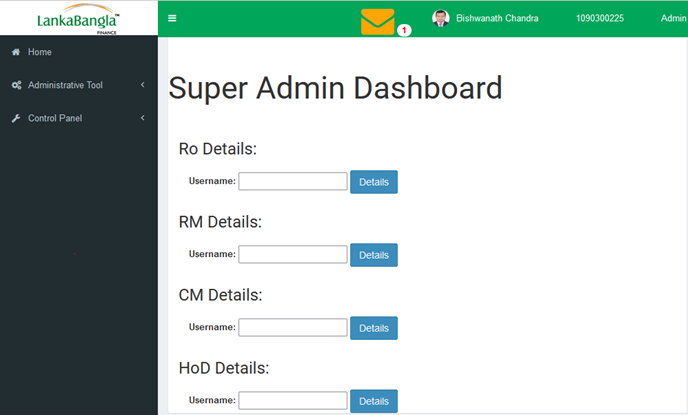
\includegraphics[width=0.75\textwidth]{image/super_admin.png}
\end{center}


% Start of Hod dashboard
\section{HoD Dashboard}
\lipsum[3-4] % Replace with details description
% end of hod dashboard



% Start of CM dashboard
\section{CM Dashboard}
\lipsum[5-6] % Replace with details description

\begin{figure}[h]
  \centering
  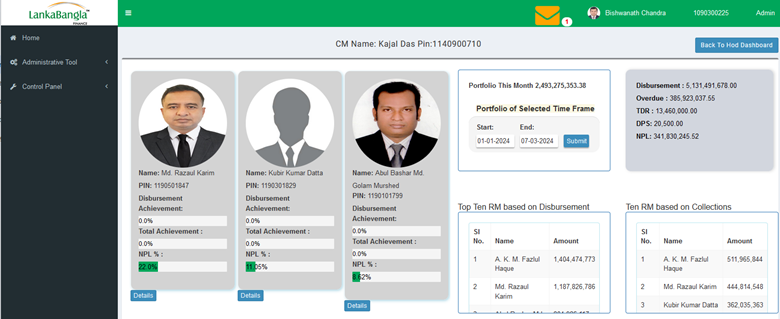
\includegraphics[width=0.75\textwidth]{image/cm_dashboard_image.png}
  \caption{CM Dashboard: This is for Cluster Manager.}
\end{figure}

\textbf{Paragraph 1:} \\
This CM dashboard provides an overview of various metrics and statistics relevant to cluster management.

\textbf{Paragraph 2:} \\
It is designed to assist Cluster Managers in monitoring and analyzing the performance and health of their clusters.

% end of CM dashboard





\section{RM Dashboard}
\lipsum[5-6] % Replace with details description


\section{RO Dashboard}
\lipsum[5-6] % Replace with details description

\end{document}
